\documentclass{beamer}
\usetheme{Boadilla}
\usepackage[utf8]{inputenc}
\usepackage[czech]{babel}
\title{Kalibrace a monitorování astročásticových teleskopů}
\author{Daniel Staník}
\institute{
SLO Upol}
\date{\today}


\begin{document}
\begin{frame}
\titlepage
\end{frame}


\begin{frame}
\frametitle{Úvod}
\begin{itemize}
 \item Detekce kosmických částic s extrémní energií (tzv. UHERC).
 \item Testování a úpravy pulzního UV kalibračního zdroje.
 \item Analýza kalibračních dat.
 \item Monitorovací systém.
\end{itemize}

\end{frame}



\begin{frame}
\frametitle{Detekce kosmických částic s extrémní energií}
\begin{itemize}
 \item energie $10^{18}$ až $10^{20}$ keV .
 \item Využití atmosféry jako kalorimetru. Vytvoření částicové a elektromagnetické spršky po zásahu energetickou částicí.
 \item Fluorescenční technika detekce - detekce deexcitačního slabého UV spektra.
\end{itemize}

\end{frame}





\begin{frame}
\frametitle{Teleskop FAST}
\begin{itemize}
 \item Fluorescenční teleskop pro detekci kosmických částic s extrémní energií (UHECR).
 \item Detekční část - čtyři fotonásobiče a superodrazná UV zrcadla.
 \item Dnes v provozu 4 prototypy.
 \item Budoucí účel - osazení velké plochy teleskopy tohoto typu a rekonstrukce spršek vyvolaných UHECR částicemi.
\end{itemize}

\end{frame}

\begin{frame}
\frametitle{Teleskop FAST}
\begin{columns}[t]
\column{.5\textwidth}
\centering
\begin{figure}[H]
\includegraphics[scale=0.3, angle = 0, origin = c]{../BachelorThesis/pictures/fastTheoretical.png}\\
\caption{Návrh teleskopu.}
\end{figure}
\column{.5\textwidth}
\centering
\begin{figure}[H]
\includegraphics[scale=0.09, angle = 0, origin = c]{../BachelorThesis/pictures/FASTReal}\\
\caption{Teleskop FAST.}
\end{figure}
\end{columns}



\end{frame}



\begin{frame}
\frametitle{Vývoj a testování kalibračního UV zdroje}
\begin{itemize}
 \item Nutnost kalibrace teleskopu jako optické soustavy. Detekční části díky různým vlivům podléhají degradaci.
 \item K tomu účelu - pulzní kalibrační UV zdroj založen na diodách. Netestován, nutnost ověření jeho funkčnosti a návrh případných úprav či jiných konceptů. K tomu účelu sestavena aparatura pro dlouhodobé měření stability zdroje.
 \item Nutno ověřit dva parametry - stabilita výkonu a stabilita geometrie pulzů. Měření prováděno v intervalu dvou týdnů. K měření výkonu užit PM16 měřící přístroj optického výkonu a k měření pulzní geometrie - fotonásobič + osciloskop.
\end{itemize}





\end{frame}

\begin{frame}
%\frametitle{Teleskop FAST}


 \begin{figure}[H]
 \centering
 \includegraphics[scale=0.05, angle = 270, origin = c]{../BachelorThesis/pictures/KarlsRuhe}
 \caption{Prototyp kalibračního zdroje.}
 \label{UVsource}
\end{figure}


\end{frame}





\begin{frame}
%\frametitle{Teleskop FAST}




 \begin{figure}[H]
 \centering
 \includegraphics[scale=0.04, angle = 0, origin = c]{../BachelorThesis/pictures/aprature1b}
 \caption{Testovací aparatura.}
 \label{UVsource}
\end{figure}


\end{frame}




\begin{frame}
\frametitle{Výsledky měření}
\begin{columns}[t]
\column{.5\textwidth}
\centering
\includegraphics[width=5cm,height=3.5cm]{../BachelorThesis/pictures/powers}\\
\includegraphics[width=5cm,height=4cm]{../BachelorThesis/pictures/Height}
\column{.5\textwidth}
\centering
\includegraphics[width=5cm,height=4cm]{../BachelorThesis/pictures/rise}\\
\includegraphics[width=5cm,height=4cm]{../BachelorThesis/pictures/Slope}
\end{columns}


\end{frame}




\begin{frame}
\frametitle{Výsledky měření}
\begin{itemize}
 \item Nalezen zásadní problém - výrazný rostoucí trend ve výkonu. Potvrzeno fotonásobičem i PM16. Pulzní geometrie - doba náběhu a sklon nemají dlouhodobý trend.
 \item Hlavní příčinnou jsou degradační procesy v samotných diodách. Viz další stránka se samotným chováním diody.
 \item Možná oprava - přidaní zpětnovazební UV detekční diody, podle které se bude upravovat proud LEDkou. 

\end{itemize}


\end{frame}



\begin{frame}
\frametitle{Degradace osamocené LED diody.}
 \begin{figure}[H]
 \centering
 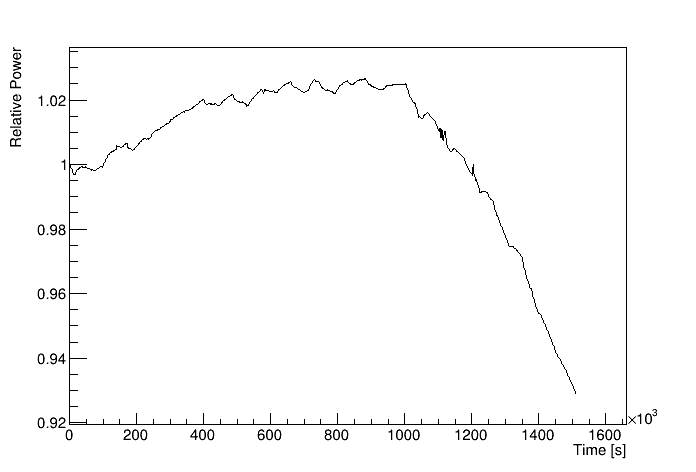
\includegraphics[scale=0.4, angle = 0, origin = c]{corrected1}
 \caption{Degradace osamocené LED diody.}
 \label{UVsource}
\end{figure}


\end{frame}



\begin{frame}
\frametitle{Optická zpětná vazba}


\begin{itemize}
 \item Zpětnovazební dioda musí být podrobena testům.
 \item Nutnost změření závislosti chování na teplotě, odezvy na pulzy a dlouhodobé stability.


\end{itemize}


 \begin{figure}[H]
 \centering
 \includegraphics[scale=0.04, angle = 180, origin = c]{../BachelorThesis/pictures/transImpedance}
 \caption{Zpětnovazební test přes transimpedanční převodník.}
 \label{UVsource}
\end{figure}


\end{frame}


\begin{frame}
\frametitle{Analýza nabraných kalibračních dat}
\begin{itemize}
 \item Při testech teleskopů nějaká kalibrační data již nabrána.
 \item Užití kalibračního UV zdroje umístěného do integrační koule, nasvěcování apertury teleskopu z různých poloh. 
 \item Hlavní účel analýzy - získání relativních kalibračních konstant pro 4 fotonásobiče.


\end{itemize}





\end{frame}

\begin{frame}
\frametitle{Ukázka analýzy}
 \begin{figure}[H]
 \centering
 \includegraphics[scale=0.2, angle = 0, origin = c]{../BachelorThesis/pictures/ukazka}
 \caption{Ukázka fitování distribucí maximální výšky kalibračních pulzů a srovnání pro 4 fotonásobiče.}
 \label{UVsource}
\end{figure}


\end{frame}





\end{document}

